% coding:utf-8

%----------------------------------------
%FOSAEBV, a LaTeX-Code for a summary of realtime image processing
%Copyright (C) 2013, Mario Felder

%This program is free software; you can redistribute it and/or
%modify it under the terms of the GNU General Public License
%as published by the Free Software Foundation; either version 2
%of the License, or (at your option) any later version.

%This program is distributed in the hope that it will be useful,
%but WITHOUT ANY WARRANTY; without even the implied warranty of
%MERCHANTABILITY or FITNESS FOR A PARTICULAR PURPOSE.  See the
%GNU General Public License for more details.
%----------------------------------------

\chapter{Einführung}

Die Bilddaten können mathematisch als Matrix beschrieben werden:
\[
	I = \left[ I_{m,n} \right] 
\]
\begin{footnotesize}
	mit $0 \leq m \leq M-1$ und $0 \leq n \leq N-1$\\\\
	\textbf{Achtung:} MATLAB verwendet das Intervall $[1,N]$ bzw. $[1,M]$\\
\end{footnotesize}

\begin{center}
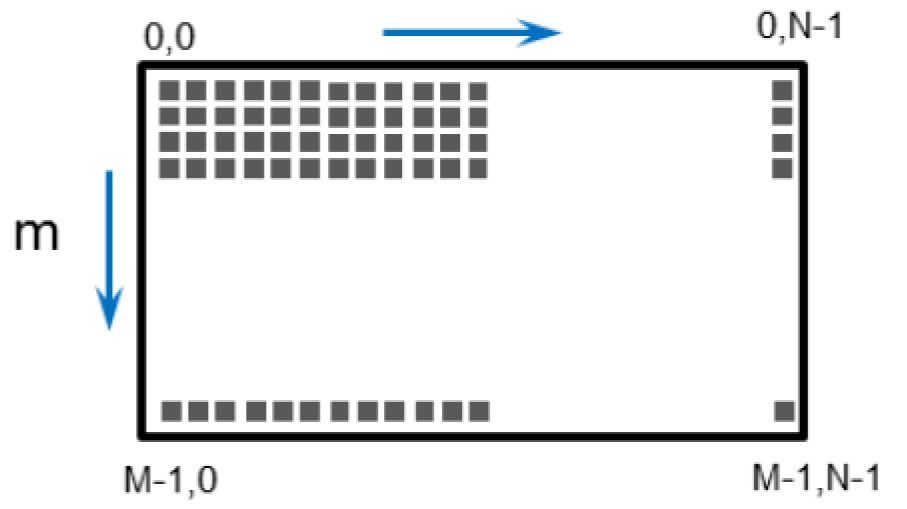
\includegraphics[scale=0.7]{./images/matrix_nomenklatur.png}
\end{center}
~\\\\

\section{Rasterung}
Die Rasterung ist ein Mass für die Detailtreue eines Bildes. 
Bei gegebener CCD- bzw. CMOS-Sensorgrösse (M x N Pixel) wird die Auflösung durch die geometrische Abbildung bestimmt.\\
\\
Dabei gelten folgende Zusammenhänge:\\
\[
	\frac{1}{g} + \frac{1}{b} = \frac{1}{f} \qquad \Leftrightarrow \qquad b = \frac{f \cdot g}{g - f}
\]\\
\begin{footnotesize}
	$f$: Brennweite\\
	$b$: Bildweite\\
	$g$: Gegenstandweite\\
\end{footnotesize}
\\
Häufig ist $g \gg b$ und es kann somit $b = f$ gesetzt werden.\\
\\
Weiter ergibt sich daraus:\\
\[
	\frac{B}{G} = \frac{b}{g}
\]\\
\begin{footnotesize}
	$B$: Bildgrösse\\
	$G$: Gegenstandsgrösse\\
\end{footnotesize}

\begin{center}
	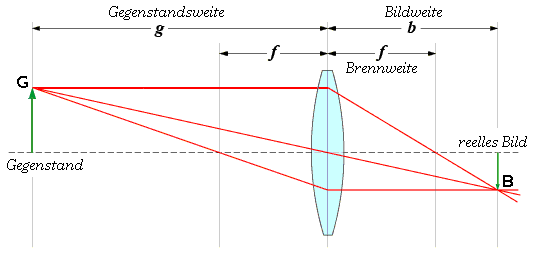
\includegraphics[scale=0.35]{./images/linse.png}
\end{center}
Auflösung bei einem Sensor mit $NxM$ Pixel Auflösung:
\[
	\begin{aligned}
		G_{b} = \frac{g \cdot W}{b \cdot N}\\
		G_{h} = \frac{g \cdot H}{b \cdot M}
	\end{aligned}
\]\\
\begin{footnotesize}
	$G_b$ : Auflösung in $\frac{mm}{Pixel}$ (Breite)\\
	$G_h$ : Auflösung in $\frac{mm}{Pixel}$ (Höhe)\\
	$W$ : Breite des Sensors $[mm]$\\
	$H$ : Höhe des Sensors $[mm]$\\
	$N$ : Horizontale Pixel\\
	$M$ : Vertikale Pixel \\	
\end{footnotesize}
\\\\

\section{Nachbarschaftsrelationen und Abstand}
Vierer-Nachbarschaft:
\begin{center}
	\begin{tabular}{|c|c|c|}
	\hline  & $m-1,n$ &  \\ 
	\hline $m,n-1$ & $m,n$ & $m,n+1$ \\ 
	\hline  & $m+1,n$ &  \\ 
	\hline 
	\end{tabular} 
\end{center}
~\\\\
Achter-Nachbarschaft:
\begin{center}
	\begin{tabular}{|c|c|c|}
	\hline  $m-1,n-1$	& $m-1,n$ 	& $m-1,n+1$  \\ 
	\hline 	$m,n-1$ 	& $m,n$ 	& $m,n+1$ \\ 
	\hline  $m+1,n-1$	& $m+1,n$ 	& $m+1,n+1$ \\ 
	\hline 
	\end{tabular} 
\end{center}
~\\\\
Euklidische Abstandsnorm:
\[
	d(I_{m,n},I_{p,q}) = \sqrt{(m-p)^2+(n-q)^2}
\]
\\
Maximum Abstandsorm:
\[
	d(I_{m,n},I_{p,q}) = max \left( \left| m-p \right|, \left| n-q \right| \right)
\]
\\\\

\section{Globale Charakterisierung von Bildern}
\subsection{Histogramm}
Das Histogramm gibt die absolute oder relative $p_I(g)$ Häufigkeit aller Grauwerte $g \in [0,255]$ eines Bildes an.\\\\
Relative Häufigkeit:
\[\begin{aligned}
	&0 \leq p_I(g) \leq 1 \qquad , \forall g\\
	&\sum_{g} p_I(g) = 1
\end{aligned}\]\\
Kumulative Häufigkeit:
\[
	h_I(g) = \sum_{g'\leq g} p_I(g') \qquad \qquad , h_I(255) = 1
\]

\subsection{Mittelwert}
\[
	\mu_I = \frac{1}{M \cdot N} \sum_{m,n}I_{m,n} = \sum_{g} g \cdot p_I(g)
\]

\subsection{Varianz}
\[
	\sigma^2_I = \frac{1}{M \cdot N} \sum_{m,n}\left( I_{m,n} - \mu_I \right)^2 = \sum_{g}(g - \mu_I)^2 \cdot p_I(g)
\]\\\\
Lösung in MATLAB:
\lstset{language=Matlab}
\lstinputlisting[firstline=3,caption=]{./Matlab/mean_sd.m}
~\\
Lösung in C:
\lstset{language=C}
\lstinputlisting[firstline=1,caption=]{./C/mean_sd.c}